% 方法主要分成三個部分

% 介紹一下方法流程

	為了提升室內定位的覆蓋率與精確度,我們方法在於增加影像定位取樣的資料,與改進傳統相機角度取樣的範圍。傳統室內影像定
位所拍出的相片只能片段的取得環境特徵,導致部分環境範圍定位準確,但沒有被拍照的範圍會定位誤差過大。本篇研究利用Kinect採集深度資料,藉由RGB-D點雲中透過虛擬相機拍攝相片
,將相片集合成影像資料庫,與待定位照片比較求出特徵點角度及位置關係作定位。

\section{虛擬影像定位流程}

	整套虛擬影像室內定位作法我們分成三大步驟來敘述:(1).採集深度資訊及虛擬環境建置,將點雲資料重合形成虛擬環境提供資料蒐集
(2).虛擬照相機設置及影像資料庫建置,拍攝虛擬相片提供定位環境資訊(3).虛擬影像定位,由相片中的特徵點對應關係求得定位位置。
圖\ref{fig:Entire System Process}為整體虛擬影像定位過程,利用Kinect 紅外深度攝影機,取得深度資訊後幫助我們做出3D的點雲環境,在環境中來作格
狀均勻分布(Grid Permutation)決定虛擬照相機的位置。因為每個照相機間距相同,代表觀察到的區域都有固定範圍,藉由規律的相機位置分布取得我們所需要的
定位資料。虛擬相片的設置在角度上的調整由深度過濾相機角度,避免相機與景物過近導致無法辨識特徵的情形發生,根據相機位置規律分布與角度篩選機制,取得比一般平面
影像定位更適合的角度與更全面的覆蓋,取出良好的定位資訊,減低之後定位所造成的誤差。
  
\begin{figure*}
\begin{center}
  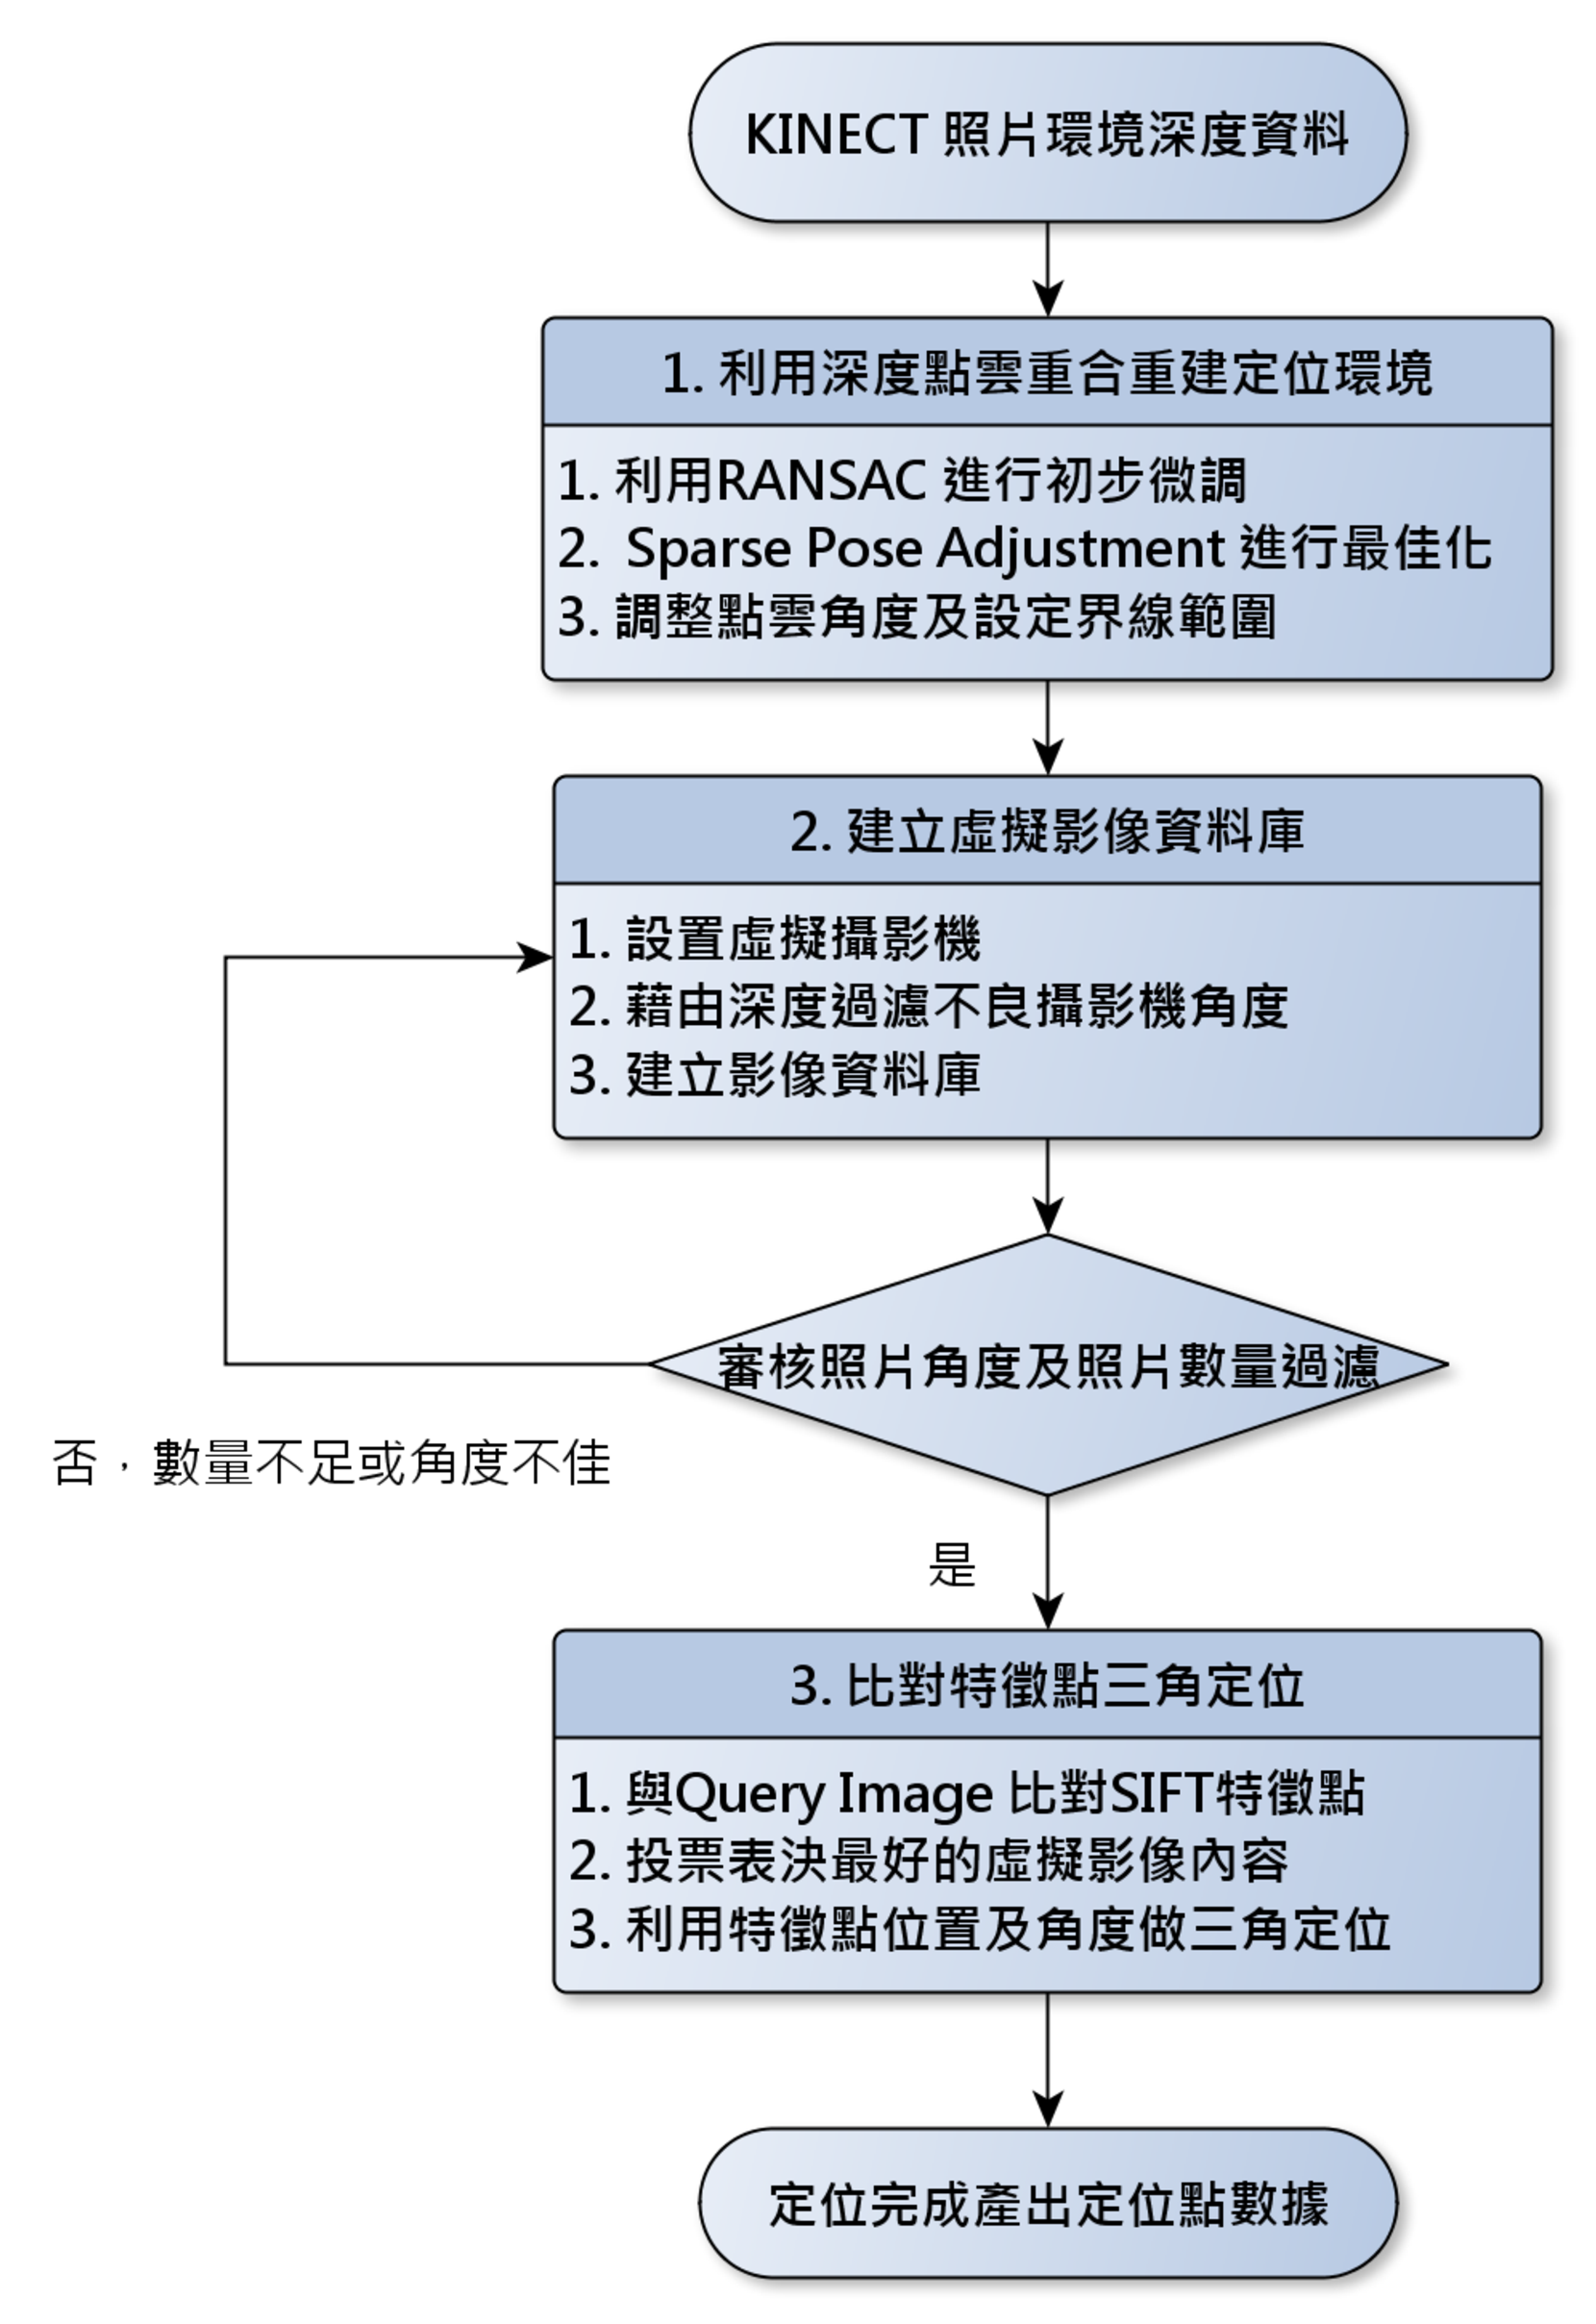
\includegraphics[width=0.8\textwidth]{figures/System_Process.eps}
  \caption{3D點雲環境座內定位整體流程圖}
  \label{fig:Entire System Process} 
\end{center}
\end{figure*}
  
% 建立 point cloud map
\section{深度資料採集與建立虛擬環境}

\begin{figure*}
\begin{center}
  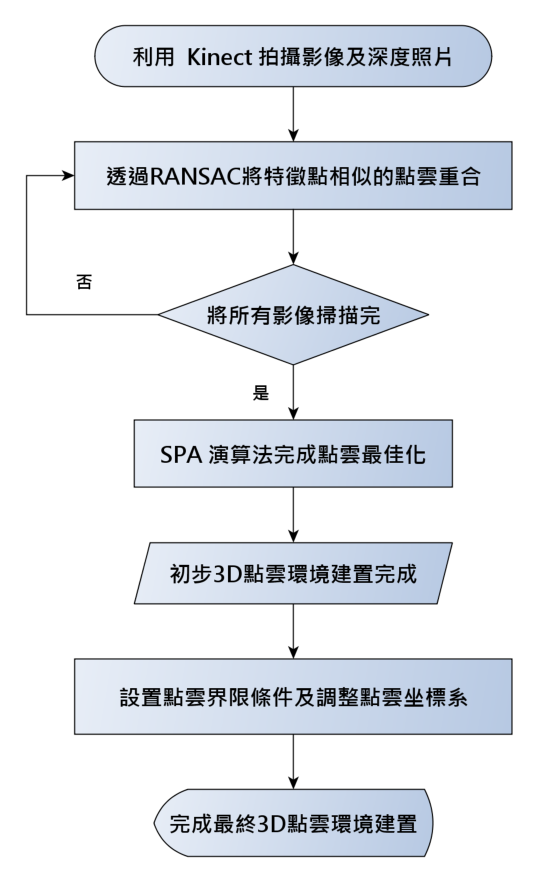
\includegraphics[width=0.6\textwidth]{figures/Environment_Building.eps}
  \caption{室內環境重建方法流程}
  \label{fig:Environment Building Process}
\end{center}
\end{figure*}

   建立RGB-D點雲環境取得定位資訊,為我們研究方法中的第一步,此舉為了增加定位資訊中的完整性。平面影像定位中的相機的位置分布通常是隨機分布,而且需要人工紀錄相機位置與角度,
如果能夠自動完成定位資料庫與增加相片的定位資訊,可以改善相片採集與建立資料庫的效率,對於定位品質的改善也有幫助。虛擬環境建立的方法首先從 Kinect 攝影機蒐集完深度照片後,利用
RANSAC比對作深度資料重合後作成初步的RGB-D點雲建置,之後透過SPA演算法完成最後點雲整體最佳化。RANSAC演算法只能做相對位置的對齊,會發生起始位置及最後位置無法重合的情況。
SPA演算法解決了RANSAC只能區域性對齊的問題,我們參考之前文獻探討中描述Visual SLAM問題中解決地圖封閉檢測的作法,將每個拍攝點的位置做紀錄找出最佳的重合路徑。重建環境方法我們分成下列幾個步驟:
   
\begin{itemize}
	\item 將每張照片經過SIFT比對後找出相似的對應特徵
	\item 將這些對應特徵點帶入RANSAC演算法中作為輸入條件,其中包括對應點的特徵與角度以及相機拍攝位置與角度,設置重複計算的次數
	\item 出來的點雲資料為區域之間的重合,沒有經過整體最佳化,會發生不一致(non-consistent)的情形,如圖 \ref{fig:Consistent_PL}所發生的情況
	\item 透過SPA將點雲做整體的最佳化,改善的情況如\ref{fig:Consistent_PL}所示
	\item 將點雲做最後微調的步驟,找出虛擬攝影機可以設置的範圍區域當作界線範圍,調整點雲角度與齊次坐標系平行
\end{itemize}
   
\begin{figure*}
\begin{center}
  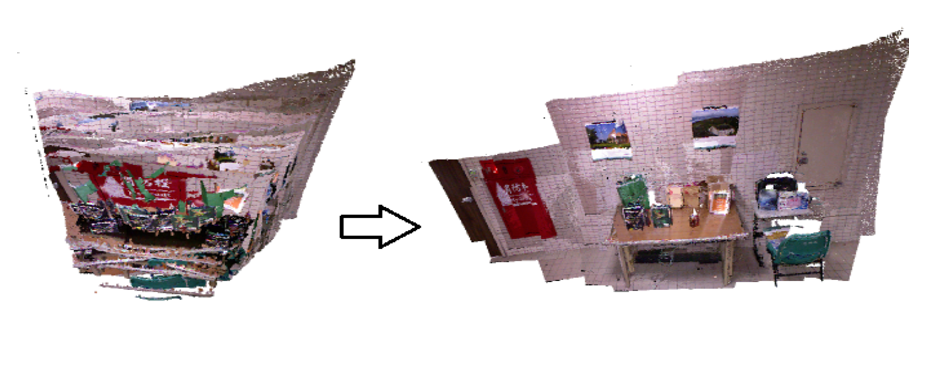
\includegraphics[width=1.0\textwidth]{figures/consistent_PL.eps}
  \caption{透過SPA演算法幫助RGB-D點雲最佳化,圖左為處理前,圖右為處理後}
  \label{fig:Consistent_PL}
\end{center}
\end{figure*}   
   
% 前3個步驟決定點雲的樣子
\subsection{RGB-D 資料採集}

% Kinect 照片組描述
	資料採集的部分,首先利用Kinect在環境中拍攝照片,取得照片深度後透過RANSAC重合這些相片位置,製作初步的點雲。深度照片取得的作法類似之前 \cite{Du2011}使用的方法,在環境中對每個景物做連續
性的拍攝,拍攝出來的照片都需要有一些相似之處,並環繞整個定位環境確保照片的組成具有連續性。當相片包含的景物越多顏色越豐富所代表所包含的特徵點越多,豐富的特徵點數量在做RANSAC
之後會有更好的重合效果。對於RANSAC而言,一個密集的點群所找到的平面會越接近真實點群的表現,所做出的轉移矩陣(Transformation Matrix)也會越精準,在進行重合時,不會
有影像疊影或者是破碎導致點雲中空、物體歪斜扭曲的現象產生。連續的環繞拍攝是為了確保每一張影像相對位置關係,不會因為順序錯誤而導至點雲破碎沒有一致性。RANSAC 怕影像排列的順序出錯,當順序不正確時會無法找出影像位置
的相對關係,在之後點雲重合所做出的景物位置會和實際環境中出現的景物位置相差甚遠。因此拍攝照片在RGB-D 資料採集的步驟中是影響最大的因素,其中因為光線的不足或是玻璃的反射等一些外在的因
素都會導致之後在建置點雲的困難,所以在作拍攝時最好都避免這些不利的因素。
          
% RANSAC 描述 
    拍攝完照片組之後,我們要依據這些照片位置與深度關係帶入RANSAC計算出重和的位置。在這之中會利用到尺度不變特徵向量(SIFT)從這些照片中取得特徵點的位置,將這些
特徵點的位置求取RANSAC,使得每一張影像都能夠在齊次坐標系中在正確的位置中重合。作法是將每張採集圖片找出來的特徵點作配對,求出這些配對關係後,將這些配對作最小平方法(Least Square Error)
求出想要的平面,根據不同平面帶入homography作出轉移矩陣(Transformation Matrix),最後得到相片位置的絕對關係,稱為 Global Pose。Global Pose包含照片三維座標以及照片在當時
拍攝的角度。在之後調整點雲角度以及制定點雲邊界都需要Global Pose的資訊,最後的影像定位過程,我們也需要Global Pose當作相片中特徵點的起始位置來協助定位。在初步的點雲建置完成後,最後我們利用之前
文獻所提到解決地圖封閉的方法,透過SPA(Sparse Pose Adjustment)將點雲作最後的調整。

	RANSAC\cite{Fischler1981}由1981年被提出,大多運用在電腦視覺上,用來預測數學模型有可能分布的狀況,透過迭代的方法使得預測的精準度增加。RANSAC的流程分為下面幾個步驟:
 \begin{enumerate}
	  \item 設定隨機挑選的inlier數量n,以及迴圈的重複次數k
	  \item 從所有的匹配中隨機挑選n個作為inliers,數量至少能夠計算出轉移矩陣
	  \item 以Levenberg-Marquardt演算法從inliers計算出投影矩陣$R_{in}$
	  \item 把inliner之外的匹配特徵帶入$R_in$,計算投影之後匹配特徵的距離,把距離小於設定門檻值得闢配都加入inliers
	  \item 紀錄所有iinliers,並比較其總數受否大於現在的最大值,如果是則更新最大值
	  \item 重複執行k次步驟2.到步驟5.,最後留下的最大值就是過濾好的特徵點,再利用Levenberg-Marquardt從這些過濾好的批被去計算出最佳轉移矩陣$R_{best}$
 \end{enumerate}

	至於n和k如何決定,可以假設每個特徵匹配為良好的機率設w,因此一開始隨機挑選的n個匹配的機率為$W^n$,其中設某個環節出錯的機率為$1-W^n$,而只要有一個是錯的,
就找不到最佳的轉移矩陣,定義p為重複執行k次之後出現出錯的機率,至少選到一次n個都為良好匹配的機率即為$1-p$,可表示為:
\begin{align} 
	1-p = (1-w^n)^k  \label{eq:failure probability} \\
	p = 1 - (1-w^n)^k \label{eq:successful probability} \\
	k = \frac{log(1-p)}{log(1-w^n)} \label{eq:RANSAC k}
\end{align}

    從(\ref{eq:successful probability})可看出,若希望p要盡可能大,則k要夠大(\ref{eq:RANSAC k}),然而k越大表示所需計算的時間也越長,因此要
先假設合理的w值,定義一個至少足以計算轉移矩陣的n值,來衡量p值與k值。

根據RANSAC所做出初步的點雲環境中,我們針對照片與照片之間相似的位置作重和,但是做出來的點雲之間會發生不一
致的情形發生,這時候需要對原始深度照片拍攝的路徑作位置的最佳化。利用SPA演算法\cite{Konolige2010},這套演算法幫助我們減少點雲環境中不一
致的情形發生,圖\ref{fig:Point Cloud Map}為經過最佳化最後所產生的點雲環境。

\begin{figure*}
%\begin{center}
  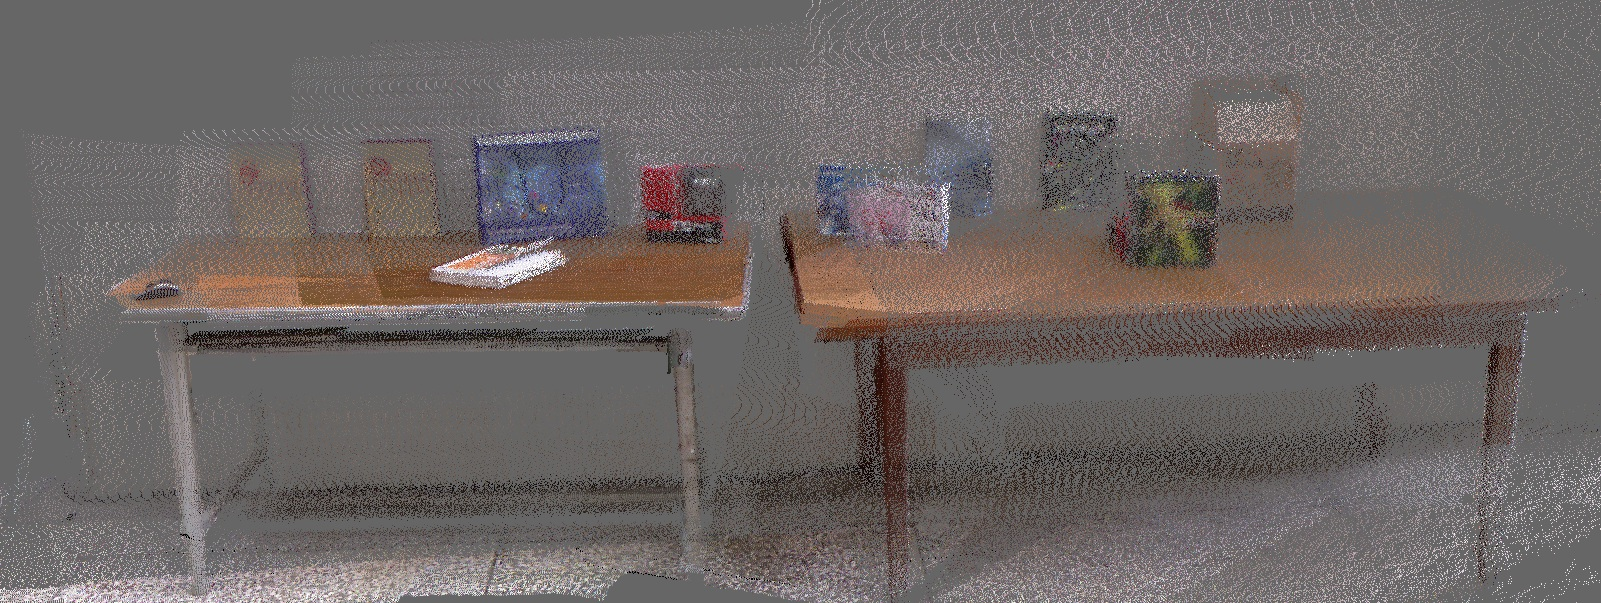
\includegraphics[width=\textwidth]{figures/3DPoint_Cloud_Map.jpg}
  \caption{初步建置好的點雲環境}
  \label{fig:Point Cloud Map}
%\end{center}
\end{figure*}

\subsection{座標系角度調整及制定邊界範圍}
     
% 後3個步驟調整點雲分布的界限範圍以及將角度調正     
    前三個步驟將點雲環境完成之後,在這個環節制定點雲的邊界範圍(Bounding Box)及調整點雲坐標系的角度,像圖\ref{fig:Bounding Box}所示。這個流程的目的是為了讓虛擬照相機
    能夠被擺放在定點雲的邊界範圍內,不會發生照相機放置在點雲環境之外而無法產生出有效的虛擬影像提供參考。尋找邊界範圍的具體做法如下,當讀入整個點雲之後,找點雲中最大及最小的$X$及$Y$座標
    ,求出位於邊界範圍的頂點座標,最後將座標值相減求出的長度即為邊界範圍的長寬。有了這些長度之後,就可以知道整個點雲環境所在的位置以及長寬的距離為何,在之後設置虛擬相機位置可防止相
    機坐落在散布點雲以外的位置,使得虛擬照片無法提供相關的定位資訊。

%%放有 Bounnding Box 的 Point Cloud 圖  
\begin{figure*}
\begin{center}
  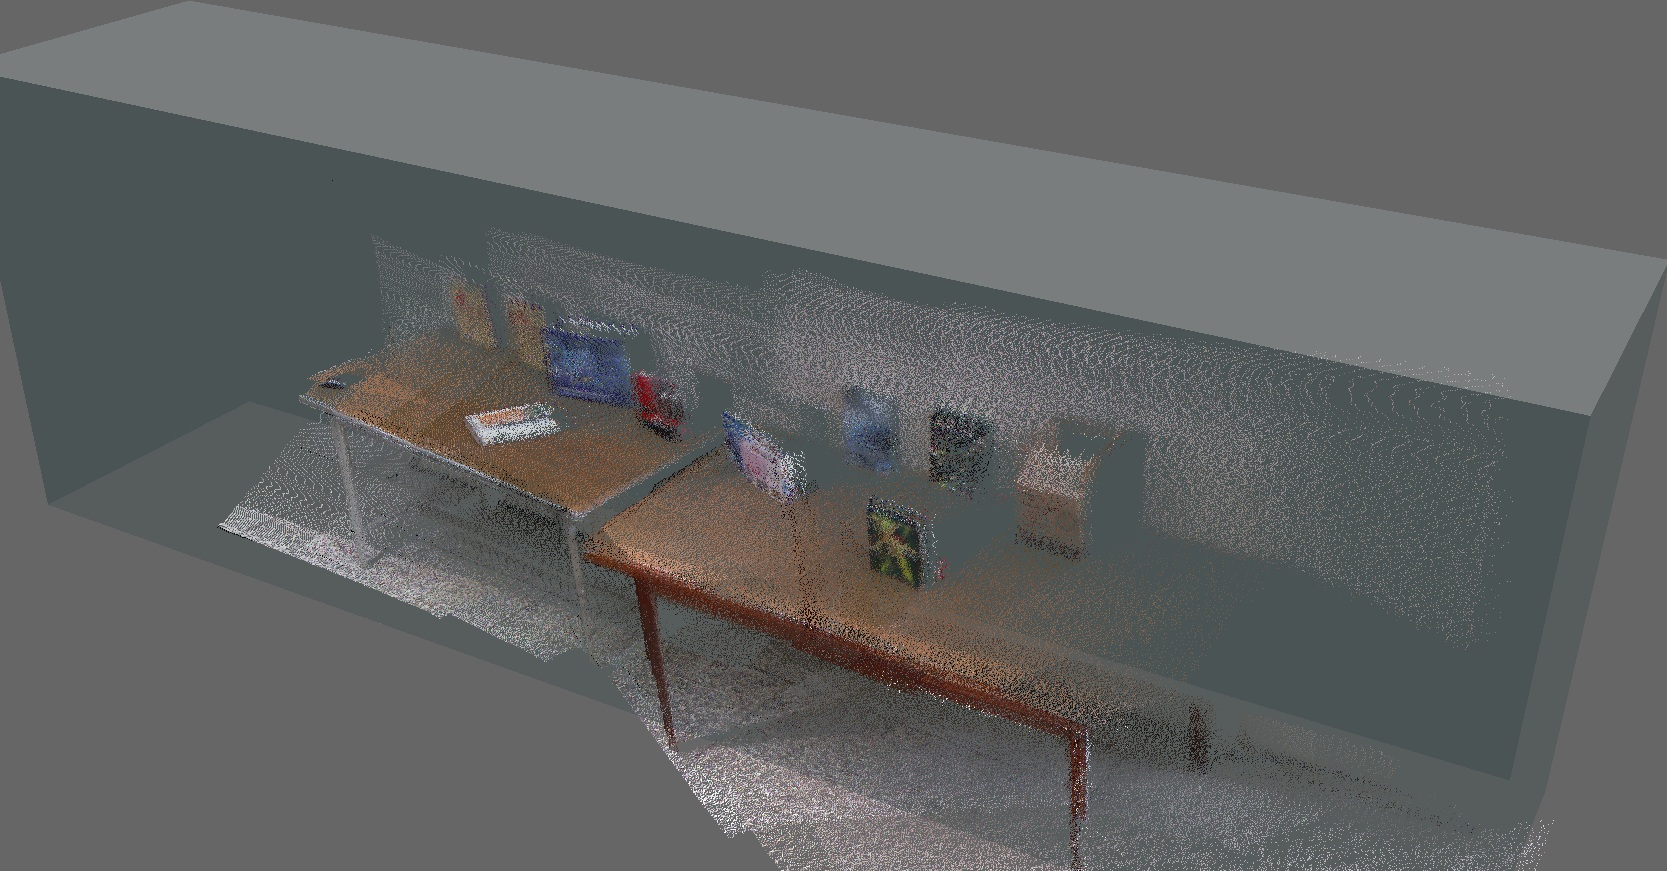
\includegraphics[width=0.5\textwidth]{figures/Bounding_Box.jpg}
  \caption{將點雲給予界限範圍}
  \label{fig:Bounding Box}
\end{center}
\end{figure*}   
    
    在制定點雲的邊界範圍之後,點雲可能會因為之前Kinect相機位置的 Global Pose 歪斜分布導致點雲也會有歪斜的狀況產生,這時候就必須將點雲作角度上的調整。這個步驟為了防止
    虛擬相機在照相時因點雲角度歪斜使得虛擬相機與真實相機的角度差異過大,減少對應的特徵點的配對關係而使得定位誤差產生。具體解決的辦法以圖\ref{fig:rotate axis}為例,
    觀察點雲是朝向哪個方向歪斜,運用Global Pose的相對位置求出Kinect攝影機角度的 $\tan \theta$,之後將點雲帶入求出來的$\theta$的旋轉矩陣旋轉至與三維座標軸平行的角度
    ,完成點雲角度調整。點雲調整的相關工作皆完成之際,就可以準備設置虛擬相機與建置資料庫的工作。

    
%放一張 攝影機 Global pose 求得後放置旋轉矩陣 的圖   
%放調整角度前的 Point Cloud 與調整角度後 Point Cloud 圖  
    
\begin{figure}
  \begin{center}
    \subfigure[使用攝影機的Global Pose求得$\tan \theta$]{\label{fig:tan}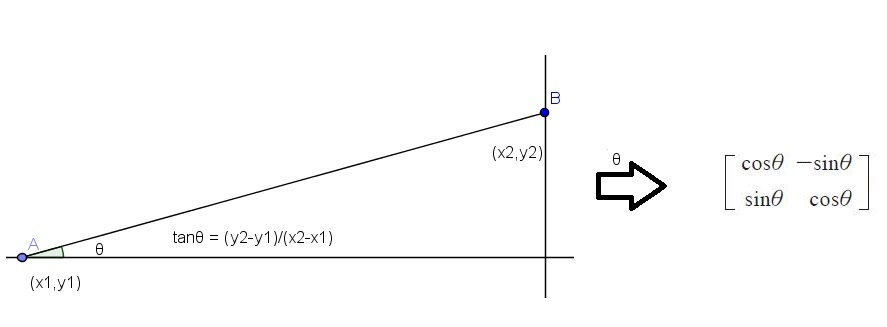
\includegraphics[width=0.65\columnwidth]{figures/Global_Pose.jpg}}
    \subfigure[坐標軸角度差異]{\label{fig:rotation result}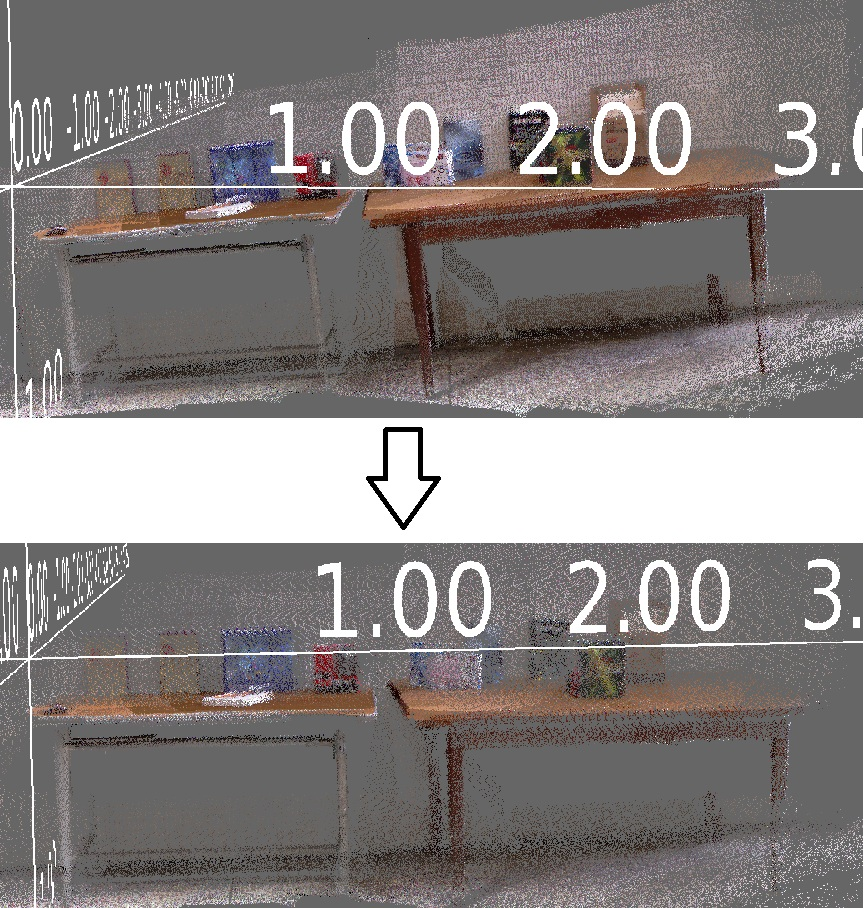
\includegraphics[width=0.33\columnwidth]{figures/Rotation_Result.jpg}}
  \end{center}
  \caption{調整點雲坐標軸角度方法 }
  \label{fig:rotate axis}
\end{figure}
    
\section{虛擬相機設置及影像資料庫建置}

\begin{figure*}
\begin{center}
  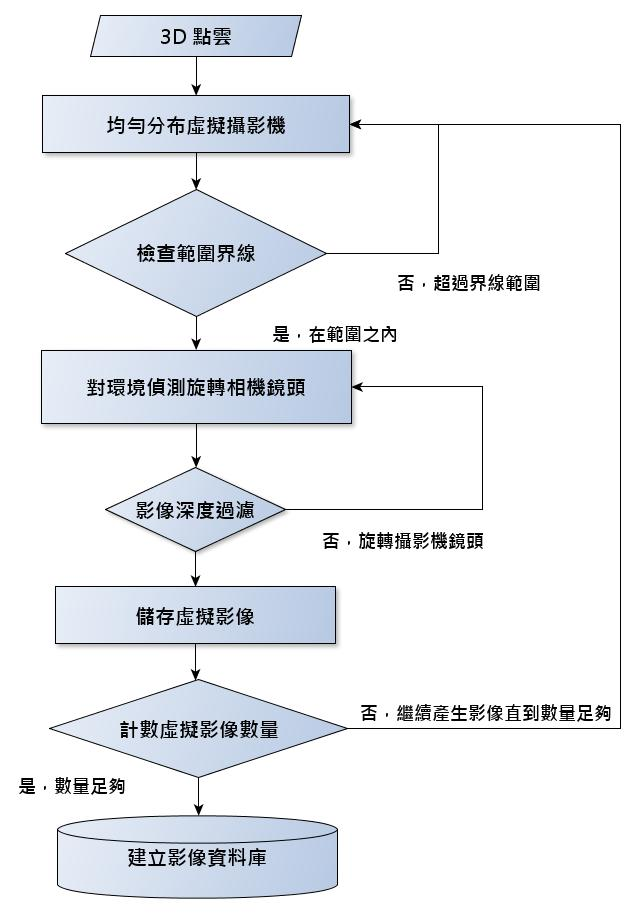
\includegraphics[width=0.8\textwidth]{figures/Virtual_Image_Database.jpg}
  \caption{影像資料庫建置流程}
  \label{fig:Environment Building Process}  
\end{center}
\end{figure*}	

	在建置完環境之後,本章節描述如何決定虛擬照相機的位置、角度以及虛擬照相機成像的原理。與一般平面影像定位方法不同的是,一般平面影像定位的資料,絕大多數都是利用隨機位
	置取得影像資料,但在我們的研究中藉由格狀分布設置虛擬照相機的位置,再隨機分布照相機拍攝的角度。依照均勻設置相機位置的方式,能夠取得比一般影像定位更完整的環境資訊,這些資訊都
	是利用點雲所產生的,不必額外拍攝相片與提供相片位置資訊作輔助。圖\ref{fig:Environment Building Process}為拍攝虛擬相片與建置影像資料庫的流程,
	在本章節裡分為四個部分描述虛擬照相機的設置流程:
	
	\begin{enumerate}
		\item 均勻分布設置虛擬攝影機
    	\item 虛擬照相機成像原理
    	\item 根據深度來調整攝影機角度
    	\item 儲存虛擬照相機圖片
	\end{enumerate}		

\subsection{虛擬相機位置分布機制}
%均勻分布設置虛擬攝影

	\begin{figure}
		\begin{center}
	    \subfigure[格狀分布虛擬相機位置]{\label{fig:Uniform_Camera_Pose}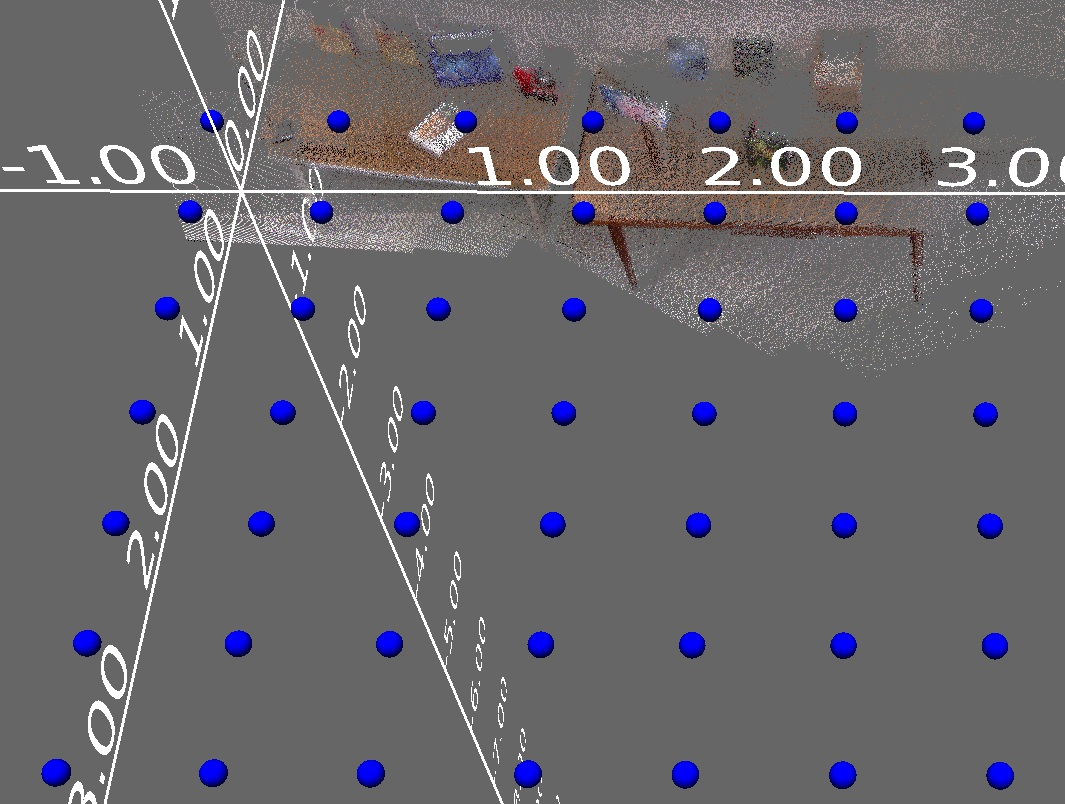
\includegraphics[width=0.45\columnwidth]{figures/VirtualCameraPose.jpg}}
	    \subfigure[隨機分布虛擬相機位置]{\label{fig:Random_Camera_Pose}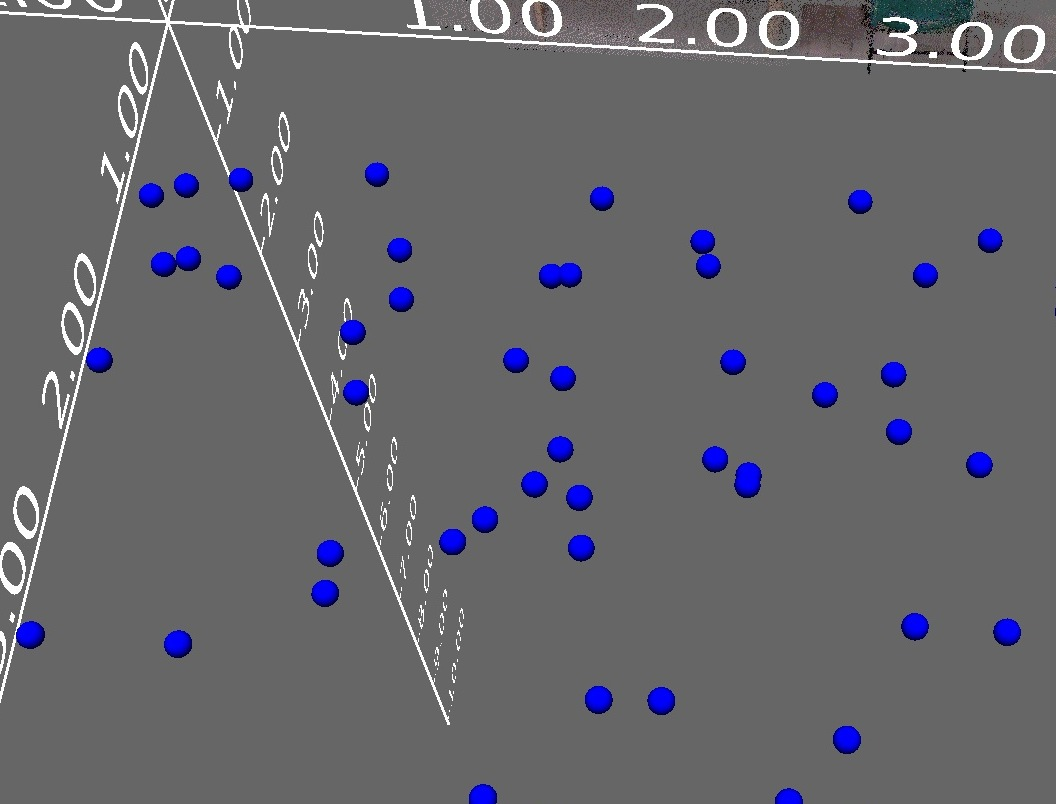
\includegraphics[width=0.45\columnwidth]{figures/Random_Virtual_Camera.jpg}}
		\end{center}
	  \caption{在點雲上設置虛擬照相機位置}
	  \label{fig:Virtual Camera Pose}	
	\end{figure}	
	
	上一個章節中,我們完成了實驗環境的建置,也就是點雲環境的資料。在這個章節中為了環境內每個景物都能被完整拍攝而取得足夠的特徵點,所以將虛擬相機位置設置成格狀分布,在每個區塊上
	設置虛擬相機。格狀分布的好處在於能夠減少相機集中在某處的情形發生,像是以圖\ref{fig:Uniform_Camera_Pose}為例,格狀分布中每個相機都有固定位置做隔。但圖
	\ref{fig:Random_Camera_Pose}相機隨機分布位置卻過於集中在黑色圓圈處,使得每個相機位置間距都不同,導致有些地方相機分布過於分散,但有些地方相機位置分布卻過於集中。
	格狀分布作法依據環境而有所改變,為了希望環境內建置50部以上的虛擬相機,我們會將環境的長度分成8個等分、寬度分成7個等分,這樣每個等
	分都會有一樣的距離間隔,可以完成56部虛擬相機擺設的位置。一般影像定位的資料來源可能只針對特定區域的特徵點作取樣,而導致特定區域內的影像定位效果非常好,但在其他區域卻沒有
	足夠的影像特徵點資料,使得定位誤差範圍過大,透過均勻分布不會有部分景物或場景沒有被拍攝到,藉以增加定位的覆蓋率與改善定位的精確度。
	
\subsection{虛擬相片成像原理}
%虛擬照相機成像原理
%
	當虛擬相機位置固定之後,接下來拍攝虛擬相片,透過虛擬相機的影像角錐來模擬相機的成像,取出影像角錐內範圍的3D點雲,投射至平面模擬真實相機所拍出的相片。在這小節裡介紹虛擬相片的成
	像原理,透過齊次坐標系,將視野調整到虛擬照相機的位置,再利用相機成像的perspective矩陣取得相機影像角錐,這個矩陣目的在於模擬相機取得視野範圍內的影像,其矩陣表示法如式子(\ref{eq:Perspective Matrix})表示:	

\begin{figure}
  \begin{center}
    \subfigure[攝影機的攝影近裁面(near)與遠裁面(far)表示]{\label{fig:glFrustum}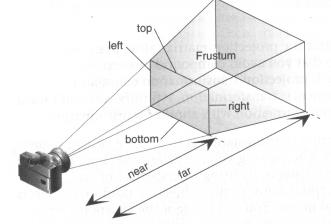
\includegraphics[width=0.45\columnwidth]{figures/Camera_image.jpg}}
    \subfigure[相似三角形表示法]{\label{fig:o_depth_interpolation}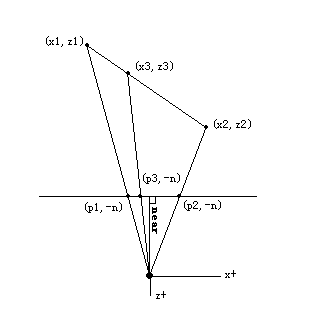
\includegraphics[width=0.45\columnwidth]{figures/o_depth_interpolation.jpg}}
  \end{center}
  \caption{glFrustrum 矩陣圖示說明}
  \label{fig:camera reference}
\end{figure}
    
	\begin{align}
	glFrustrum = \left( \label{eq:Perspective Matrix}
		 			\begin{array}{cccc}
		 			\frac{2near}{right - left} & 0 & \frac{right + left}{right - left} & 0 \\
		 			0 & \frac{2near}{top - bottom} & \frac{top + bottom}{top - bottom} & 0 \\
		 			0 & 0 & -\frac{far + near}{far - near}  & -\frac{2far \times near}{far - near} \\
		 			0 & 0 & -1 & 0 \\
		 			\end{array}
		 		\right)
	\end{align}
	
	                    
	將三維座標轉為齊次座標後,如圖\ref{fig:glFrustum}利用攝影機的攝影近裁面(near)與遠裁面(far)的相似三角形來推導出矩陣,這矩陣會將角錐內深度在
	$[-1,1]$之間的點雲投影至平面。這部分攝影機的焦距設定,
	以及解析度都參照Kinect紅外深度攝影機的參數設定。要解釋如何求出perspective矩陣,需要用到兩項條件來說明:(1) 證明$\frac{1}{z}$為線性關係,
	(2) 將(1)所求出的公式帶入投影座標求出矩陣關係式。
	
	(1) 證明$\frac{1}{z}$為線性關係:
	
	根據圖\ref{fig:o_depth_interpolation}所示,由相似關係三角形得出的關係式:
	
	\begin{align}
		\label{eq:Similar Triangles}
		p = \frac{-n}{z} \times x		 		
	\end{align}
	
	而我們知道直線關係式為 $y = ax + b$,將式(\ref{eq:Similar Triangles})帶入直線關係式得出	
	\begin{align}
		\label{eq:p equation}
		p = \frac{n}{a} (\frac{z}{b} - 1)
	\end{align}
	
	由圖\ref{fig:o_depth_interpolation}可得知$(p_1,p_2,p_3)$在同一條線上,利用其線性關係,將式(\ref{eq:p equation})帶入$p_3 = tp_2 +(1-t)p_1$得出:	
	\begin{align}
		\label{eq:p is linear}
		\frac{n}{a} (\frac{b}{z_3} - 1) = t \frac{n}{a} ( \frac{b}{z_1} - 1) + (1-t)\frac{n}{a} (\frac{b}{z_2} - 1)
	\end{align}
	
	化簡式(\ref{eq:p is linear})後得出:
	\begin{align}
		\frac{1}{z_3} = t \frac{1}{z_1}  + (1-t)\frac{1}{z_2} 
	\end{align}
		
	在證明$\frac{1}{z}$為線性關係後,接下來由(1)所推導的結果帶入persepctive攝影角錐中
		
	(2) 將(1)所求出的公式帶入投影座標求出矩陣關係式:
	
	在這個階段中,要把之前求出的關係式都帶到投影座標內,我們假設$(x, y, z, w)$為攝影機座標,$(x', y', z', w')$為投影座標,而$(P_x,P_y,P_z,P_w)$為攝影角錐內的座標,
	以圖\ref{fig:glFrustum}為例,t=top, l=left, r=right, b=bottom,對於x,y其中關係式可以寫為:	
	\begin{align}
	\label{eq:x,y is linear}
		x' = \frac{-nx}{z}  \quad y' = \frac{-ny}{z}
	\end{align}
	
	帶入攝影角錐內的投影座標$(P_x,P_y,P_z,P_w)$,將其縮放到可視範圍$[-1,1]$之間,得出:	
	\begin{align}
	\label{eq:P in perspective}
		\frac{1-P_x}{1-(-1)} = \frac{r-x'}{r-l} \quad 	\frac{1-P_y}{1-(-1)} = \frac{t-y'}{t-b}
	\end{align}
	
	化簡式(\ref{eq:P in perspective})後得出:
	\begin{align}
		P_x = \frac{2x'}{r-l} - \frac{r+l}{r-l} \quad   P_y = \frac{2y'}{t-b} - \frac{t+b}{t-b}
	\end{align}
	
	帶入$x',y'$在式(\ref{eq:x,y is linear})中所得到的結果:
	\begin{align}
		P_x = \frac{2n}{r-l} (-\frac{x}{z}) - \frac{r+l}{r-l} 	\quad	P_y = \frac{2n}{t-b} (-\frac{y}{z}) - \frac{t+b}{t-b} 
	\end{align}
	
	已知$P_Z$與$\frac{1}{z} $呈現性關係,設$P_z = \frac{a}{z}+b$,求a與b。已知兩點$(-n,-1),(-f,1)$再近裁面中,所以得出下列結果:
	\begin{align}
		a = \frac{2nf}{f-n} \quad b = \frac{f+n}{f-n} \\
		P_z = \frac{2nf}{f-n}(\frac{1}{z}) + \frac{f+n}{f-n} 
	\end{align}
	
	把$P_x, P_y$與$P_Z$轉成齊次坐標系得出:
	\begin{align}
		\left\{
		\begin{array}{ccc}
		-zP_x = \frac{2n}{r-l}x + \frac{r-l}{r+l}z  \\
		-zP_x = \frac{2n}{t-b}x + \frac{t+b}{t-b}z  \\
		-zP_z = -\frac{2nf}{f-n} - \frac{f+n}{f-n}z \\
		w = -z\\
		\end{array}
		\right.
	\end{align}
	
	上述為perspective矩陣式子所推導的過程,我們將攝影角錐內的點雲投影成平面,存取虛擬影像。在存取完虛擬影像後,根據物體距離攝影機遠近或太靠近點雲邊界,判斷相機位置是否會
	太逼近點雲環境內的景物或太靠近點雲邊界。如何判斷利用影像內的平均深度,決定相機角度的選擇是否適當,增加資料庫內影像定位資料的關聯性,這部分會在下面的章節作說明。
	
\subsection{攝影機角度過濾機制}
%根據深度來調整攝影機角度
%

	\begin{figure*}
	\begin{center}
	  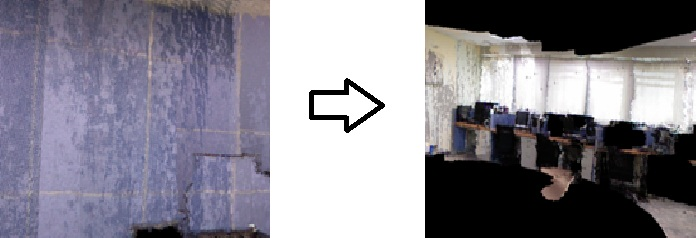
\includegraphics[width=1.0\textwidth]{figures/Depth_Filter.jpg}
	  \caption{根據物體距離鏡頭遠近來調整方位}
	  \label{fig:Depth_Filter}
	\end{center}
	\end{figure*}

	在虛擬相機的圖片擷取出來後,因為拍照的相機深度過淺或者位於點雲的邊界範圍上,而導致拍攝的景物無法辨識,這時候我們利用深度過濾的機制來將照相機取得角度作過濾。
	一般深度buffer的表示方式分為z-buffer與w-buffer兩種,我們從兩種不同的深度分辨方式作探討:
	
	關於深度的計算方式,利用齊次座標軸$(x,y,z,w)$表示三維座標軸$(x',y',z')$的點,以圖\ref{fig:glFrustum}為例,
	t=top, l=left, r=right, b=bottom,其空間關係的表示法為:
	\begin{align}
		\left\{
		\begin{array}{ccc}
		x' = x /w \\
		y' = y /w \\
		z' = z /w \\
		\end{array}
		\right.
	\end{align}
	
	根據圖\ref{fig:glFrustum}的示意圖表示,$Z_n = near$面的z範圍,$Z_f = far$面z範圍,$w = \frac{2 \times Z_n}{right-left}$,$Q = \frac{Z_f}{Z_f - Z_n}$ 由z座標求得w縮
	放的比例,式子可以寫為:
		
	\begin{align}
		w = \frac{Q\times Z_n}{(Q-Z)}
	\end{align}			
	
	z-buffer 是保存經過perspective投影矩陣投影後的 z 坐標,投影後的物體會產生近大遠小的效果,所以距離眼睛比較近的地方,z 坐標的分辨率比較大,而遠處的分辨率則比較小。換句話說,投影後的
    z 坐標在其值的分布上,從景物對眼睛的物理距離變化為非線性變化(即非均勻分佈),這樣的一個好處是近處的物體得到了較高的深度辨識,但是遠處物體的深度判斷可能會出錯。 
    
    w-buffer 保存的是經過投影變換後的齊次坐標系中的 w 坐標,而 w 坐標通常跟世界坐標系中的 z 坐標成正比,所以投影至平面之後,其值依然是線性分佈的,這樣無論遠處還是近處的物體,都
    有相同的深度分辨率,這是它的優點,則缺點就是不能用較高的深度分辨率辨識近處的物體。
    
    針對兩種不同的深度Buffer比較,因為我們的做法是來判別景物是否距離鏡頭過近,所以在深度判斷上是採用z-Buffer的作法,當我們判斷鏡頭與物體距離實際深度小於0.9時,相機鏡頭會
    轉向180度,也就是正後方來重新拍攝,避免鏡頭距離物體過近或是拍攝到點雲邊界,導致影像模糊或殘缺的情形發生,在此也增加影像資料庫內定位資料的關聯性。

\subsection{儲存虛擬相機影像建立資料庫}
%儲存虛擬照相機圖片
%
	當決定虛擬相機拍攝的位置與角度之後,拍攝虛擬影像將資料儲存至影像資料庫中,來進行影像定位的前置作業。虛擬影像儲存是透過虛擬相機鏡頭裡的每一個像素寫入相片裡頭,主要作法
	如下。當從 z-buffer 讀出來的深度錯誤時,代表這個像素對應在點雲上是一個黑點或者是說根本沒有點雲的資訊,以黑色作為代表,在深度辨識沒有錯誤有值讀入時,則代表它具有實際點雲的
	資料,我們找出點雲對應的顏色資訊,寫入圖檔裡,完成初步的虛擬相片。根據上述的方法,會遇到透視的問題,就是說原本不應該出現的景物會出現在正確位置之前,像
	圖\ref{fig:interpolation}在圓圈中所表示,原本在之後的物體跑在正確位置之前,像是穿透障礙物一樣,圓圈中不該出現桌子的地方,因為發生了透視的現象而出現了桌子。我們所改進的方法
	為根據周圍的深度來做內插補強。
	
%放一個內插補強前後的差異圖	 
	\begin{figure*}
	\begin{center}
	  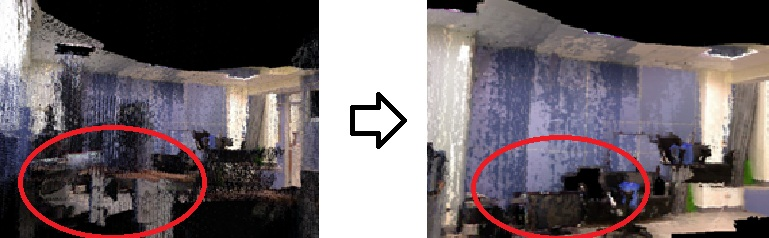
\includegraphics[width=1.0\textwidth]{figures/Depth_Interpolation.jpg}
	  \caption{內差法補強前後的差異圖}
	  \label{fig:interpolation}
	\end{center}
	\end{figure*}	
	
	虛擬影像的資料量因環境而變,主要根據虛擬相機的Global Pose在每個位置上相隔120度拍攝兩張不同相片,一般情況下點雲環境會有40組以上的虛擬相機位置,所以總共會有80張的以上的虛
	擬影像。藉由這些虛擬影像,取得定位環境在內的不同位置與不同角度的景物資料,根據先前所描述的相機設置方式與角度上的篩選,比起一般的平面影像定位資料庫多出了更豐富的特徵點資訊。之後會在
	室內定位實驗證實定位改善的成果,根據相機位置設置的方式以及距離特徵點的遠近會對定位帶來什麼樣的影響,留在實驗部分進行討論。在定位方法的最後一個章節,介紹如何利用虛擬影像特徵點
	進行三角定位。

\begin{figure*}
\begin{center}
  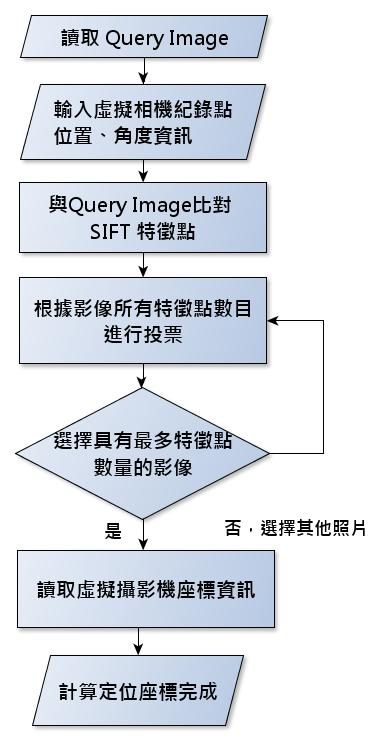
\includegraphics[width=0.6\textwidth]{figures/Localization_Process.jpg}
  \caption{虛擬影像定位整體流程圖}
  \label{fig:Lolcalization Process}  
\end{center}
\end{figure*}

\section{虛擬影像特徵點三角定位}
% 定位的決策

	在定位的流程中,讀取待定位的圖片,根據定位照片中特徵點數量的多寡,投票表決找出最合適的虛擬影像,參照虛擬影像所在的相機位置來定位,節省利用三角定位(Triangulation)所需的
	時間。
	比較與之前不同的影像資料庫建置方法,改善許多平面影像所無法定位的地方,增加定位的覆蓋率。圖\ref{fig:Lolcalization Process}為影像定位的整體流程,在定位的程序上,主要
	會分成3個階段:
		\begin{enumerate}
			\item 導入虛擬相機坐標位置作參考
    		\item 尋找特徵點並找出最多的特徵點投票選出位置
    		\item 利用虛擬照相機位置來定位
		\end{enumerate} 
		
\subsection{導入虛擬相機坐標位置作參考}	
%前置作業處理

	在定位之前,會先輸入虛擬照相機的Global Pose。虛擬照相機的Global Pose記錄檔格式包含每個虛擬相機的$X,Y,Z$座標以及相機的角度位置,當流程執行到特徵點定位時,就會
	需要參考到虛擬相機的位置。這些Global Pose的紀錄為先前在制定相機位置分布與角度時所記錄下來的資訊,等同於平面影像定位中真實相機的位置及角度資訊。藉由這些資訊得知虛擬
	影像所在位置,提供虛擬相片中特徵點比對前參考的起始位置。
		
\subsection{尋找特徵點並找出最多的特徵點投票選出位置}	
%尋找特徵點並找出最多的特徵點投票選出位置

	在前置作業完成之後,接下來利用資料庫中所有的虛擬相片進行特徵點配對,在配對的過程中,將每張照片所擁有配對關係的特徵點數量記錄下來。如先前所述,我們利用SIFT比對特徵
	找出與待定位相片中對應的特徵點,提供之後定位所需要的特徵點位置資訊。當資料庫片的照片中特徵點的數量越多,代表與待定位的照片有越密切的關係,表示相片出現的景物與待定
	位相片有很大的重複性,相當於相片在相機位置附近或是相片拍攝角度與當時待定位相片所拍攝的角度一致,最好的情形是都符合上述兩種情況,所以在資料庫中,我們選出們定位最有幫助
	的相片,相當於最多特徵點數量的虛擬相片。選出虛擬相片後,參考當時拍攝虛擬照片的相機編號,根據編號比對找出相機所在的位置,利用虛擬相機的Global Pose當作初步定位位置的
	參考起始點。
	
	\begin{figure}
    	\begin{center}
    		\subfigure[根據虛擬相片找出的特徵點]{\label{fig:SIFT_Descriptor}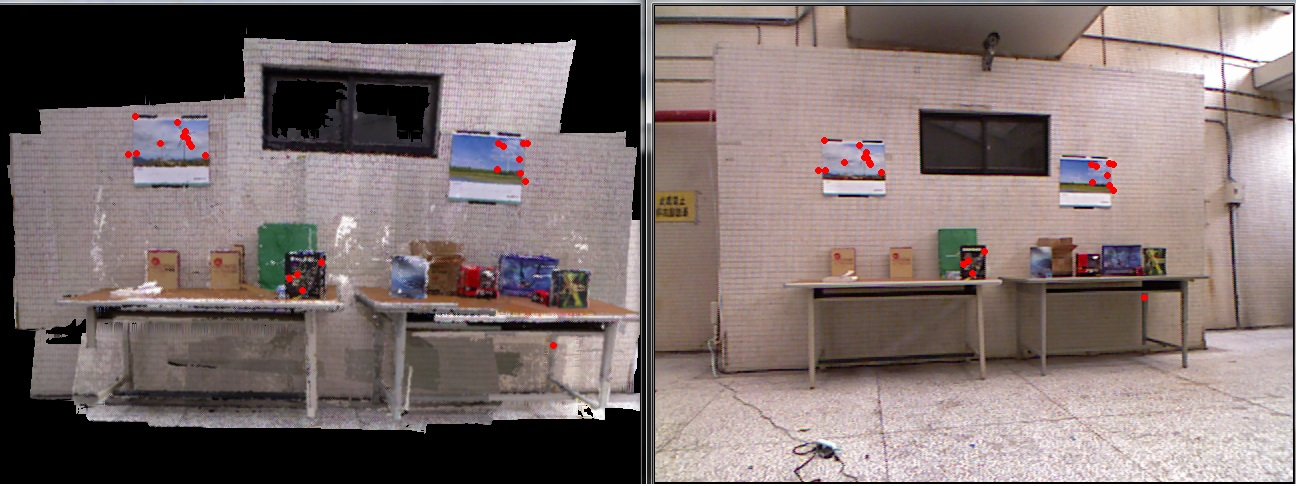
\includegraphics[width=1\columnwidth]{figures/SIFT_Descriptor.jpg}}
    		\subfigure[根據實際相片找出的特徵點]{\label{fig:SIFT_Descriptor2}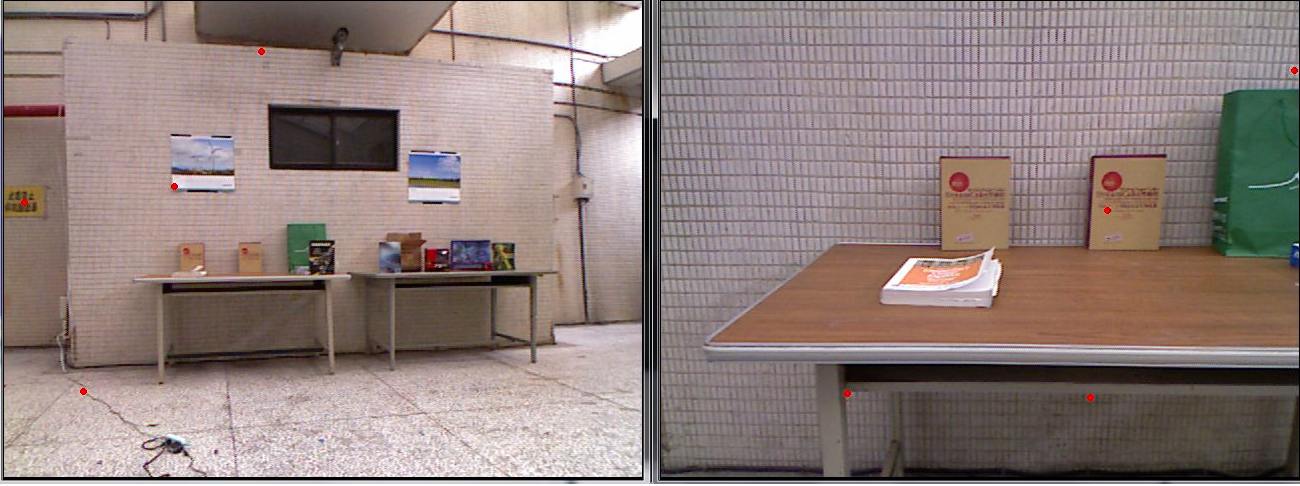
\includegraphics[width=1\columnwidth]{figures/SIFT_Descriptor(2).jpg}}
    	\end{center}
    	\caption{特徵點比較差異圖,從圖中差異得知一般相機在與景物距離較遠的情形下,會有較少的特徵比對結果,虛擬相片因為模擬當時待定位所拍攝相片的位置取景,有較高的特徵相似程度}
    	\label{fig:SIFT_Descriptor_Match}
    \end{figure}
	
	如圖\ref{fig:SIFT_Descriptor_Match}所示,特徵點的分布跟環境景物的分布有著密切的關係,在我們的作法上藉由虛擬照片找到距離特徵景物遠的待定位照片,卻可以比一般的照片找出更
	多的特徵點。利用虛擬照片我們可以有效的找出更多的環境特
	徵,在之後的定位上不管是覆蓋率或是精準度都有一定程度的提升。

\subsection{利用虛擬相機位置來定位}
%利用虛擬照相機位置來定位

	最後定位我們利用虛擬相機的位置來當作定位的參考位置,在利用虛擬相機的位置來定位與一般影像定位不同的地方在於三角定位的使用。在這裡我們先解釋一般三角定位的流程:
	\begin{enumerate}
			\item 找出特徵點對於鏡頭的夾角
    		\item 利用夾角帶入餘弦定理(Cosine Law)求出特徵點所距離鏡頭位置的長度
    		\item 利用已知的長度求出待定位圖片的位置
	\end{enumerate}
	
	\subsubsection{找出特徵點對於鏡頭圖片的夾角}
	
	\begin{figure*}
	\begin{center}
	  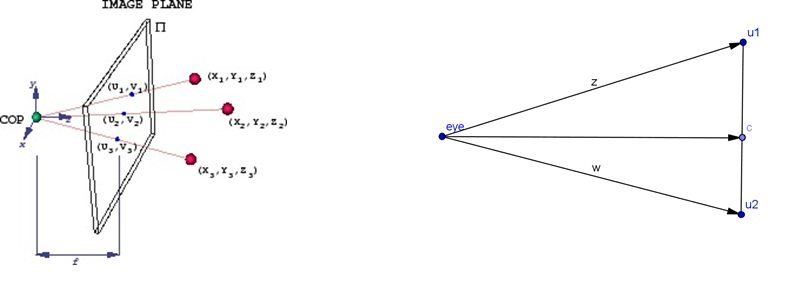
\includegraphics[width=1.0\textwidth]{figures/Included_Angle.jpg}
	  \caption{相機與特徵點的夾角示意圖}
	  \label{fig:Included Angle}
	\end{center}
	\end{figure*}
	
	在 \ref{fig:Included Angle} 當中我們要先求得$\vec{z}$與$\vec{w}$的長度,當我們知道$\vec{U_1}$與$\vec{U_2}$之後,帶入下列求解的算式:
	\begin{align}
		\left\{
		\begin{array}{cccc}
		\vec{z} = (u_{1x} - c_x)\vec{u} + (v_{1y} - c_y)\vec{v} + \vec{f}d\\
		\vec{w} = (u_{2x} - c_x)\vec{u} + (v_{2y} - c_y)\vec{v} + \vec{f}d\\
		\end{array}
		\right.
	\end{align}
	在這之中,f 為焦距向量,d 為深度。	
	
	我們得到$|z|$與$|w|$的長度,在圖\ref{fig:Included Angle}我們知道$|u|$的長度之後,再帶入餘弦定理求得角度$\alpha$的夾角:
	\begin{align}
		|\vec{u}|^2 = |\vec{z}|^2 + |\vec{w}|^2 - 2zwcos\alpha
	\end{align}	
	
	\subsubsection{利用夾角帶入餘弦定理 (Cosine Law) 求出特徵點所距離鏡頭圖片位置的長度}
	
	\begin{figure}
    \begin{center}
    		\subfigure[角度$\alpha$對於夾角$\vec{z}$與$\vec{w}$示意圖]{\label{fig:Included Angle(2)}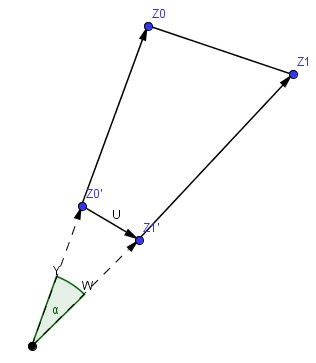
\includegraphics[width=0.3\textwidth]{figures/Included_Angle(2).jpg}}
    		\subfigure[利用夾角帶入餘弦定理 (Cosine Law) 求出特徵點所距離鏡頭圖片位置的長度]{\label{fig:Localization}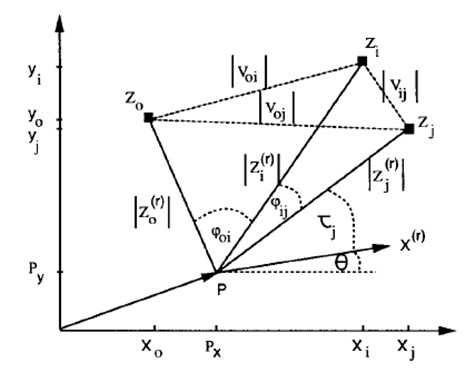
\includegraphics[width=0.6\textwidth]{figures/Localization.jpg}}
    \end{center}
    \caption{定位點夾角與長度向量關係示意圖}
    \label{fig:Localization Relationship}
    \end{figure}


	由圖\ref{fig:Localization Relationship} 我們可以知道$\varphi _{oi}$與$\varphi _{ij}$也知道$|V_{oi}|$, $|V_{oj}|$與$|V_{ij}|$的長度,藉由餘弦定理可以推出下列算式:
	
	\begin{align}
		\left\{
		\begin{array}{cccc}
		|V_{oi}|^2 = |Z_o^{(r)}|^2 + |Z_i^{(r)}|^2 - 2|Z_o^{(r)}||Z_i^{(r)}|\varphi _{io}\\
		|V_{oj}|^2 = |Z_o^{(r)}|^2 + |Z_j^{(r)}|^2 - 2|Z_o^{(r)}||Z_j^{(r)}|\varphi _{jo}\\
		|V_{ij}|^2 = |Z_i^{(r)}|^2 + |Z_j^{(r)}|^2 - 2|Z_j^{(r)}||Z_j^{(r)}|\varphi _{ij}\\
		\end{array}
		\right.
	\end{align}	
	
	其中(r)代表從定位點 P 所觀測出的位置與視角。	
	
	當我們解出$|Z_o|$,$|Z_i|$以及$|Z_j|$之後,根據圖上的座標表示法,我們最後帶入式子(2.7)中求解
	
	\subsubsection{利用已知的長度求出待定位圖片的位置}
	
	\begin{align}
		\left\{
		\begin{array}{cccc}
		|Z_o^{(r)}| = (x_o - p_x)^2 + (y_o - p_y)^2\\
		|Z_i^{(r)}| = (x_i - p_x)^2 + (y_i - p_y)^2\\
		|Z_j^{(r)}| = (x_j - p_x)^2 + (y_j - p_y)^2\\
		\end{array}
		\right.
	\end{align}	
	
	我們利用上述式子整理可得出下列式子:
	
	\begin{align}
		\left\{
		\begin{array}{cccc}
		|Z_o^{(r)}|^2 - |Z_i^{(r)}|^2 = X_o^2 - X_i^2 + 2p_x(x_i - x_o) + y_o^2 - y_i^2 + 2p_y(y_i-y_o)\\
		|Z_o^{(r)}|^2 - |Z_j^{(r)}|^2 = X_o^2 - X_j^2 + 2p_x(x_j - x_o) + y_o^2 - y_j^2 + 2p_y(y_j-y_o)\\
		\end{array}
		\right.
	\end{align}	
	
	在依照(2.7)式子兩兩相減,可得出六項聯立方程組,(2.8)為其中的兩項,在式子當中我們求出$p_x$及$p_y$則為我們想要定位之座標。當然所有的特徵點會超過
	3點以上,這些將些的餘弦等式利用最小平方法求解,得出我們想要的定位結果。
	
    上面為傳統2D平面影像根據特徵點的定位流程,我們根據虛擬影像也可以與待定位照片根據特徵點定位。但是虛擬影像為3D投影回2D的平面影像,在座標空間表示
    會面臨到投影所產生的誤差,再者點雲所見出的環境深度因為Kinect深度攝影機本身偵測的深度也會產生誤差,由虛擬影像跟平面影像特徵點利用式子求解比平面
    影像定位求解來的誤差更大。根據這點,我們利用虛擬相機的位置來當參考的定位點,當我們找出最多特徵點的虛擬照片後,我們還是利用虛擬影像作三角定位,當
    所求的定位點與虛擬相機絕對距離超過70公分,我們就利用虛擬相機位置做最後定位點,否則則三角定位的位置則為最後定位完成的結果。
    
    會這樣做的理由基於每個相機的x軸距離與y軸距離是50公分,為均勻分布,所以假定最大的平均定位誤差就為$\sqrt{x^2+y^2}=70.7$公分,當定位位置與相機距離超過
    平均誤差距離,我們會捨棄三角定位的結果,改以最多特徵點的虛擬相機位置為最終的成果。

%		之後的章節,我們將與傳統影像定位的方法作比較,根據在特徵點固定下的環境與一般室內定位環境作定位結果探討。